\documentclass[acmtog]{acmart}
\usepackage[ngerman, english]{babel}
\usepackage[utf8]{inputenc}
\usepackage[T1]{fontenc}
\usepackage{enumitem}

\copyrightyear{2024}
\acmYear{2024}
\citestyle{acmauthoryear}

\usepackage[figurename=Fig.]{caption}
\setcopyright{none}
\makeatletter
\renewcommand{\fnum@figure}{Abb. \thefigure}
\makeatother
\addto\captionsngerman{\renewcommand{\figurename}{Abb.}}
\settopmatter{printacmref=false} % Removes citation information below abstract
\renewcommand\footnotetextcopyrightpermission[1]{} % removes footnote with conference information in first column

\usepackage[cache=false]{minted}
\setminted{
    breaklines=true,
    samepage=true,
}
\usepackage[minted, most]{tcolorbox}
\usepackage{url}

\usepackage{tikz}
\usetikzlibrary{arrows, arrows.meta, positioning}


\begin{document}

\hypersetup{
	colorlinks,
	allcolors=blue,
	citecolor=.,
}

\title{Requirements Engineering: User Stories und Epics in Vorgehensmodellen}

\author{Jonas Pohl}
\authornote{Alle Studierenden trugen zu gleichen Teilen zu dieser Arbeit bei.}
\author{Mose Schmiedel}
\authornotemark[1]
\author{Antonia Swiridoff}
\authornotemark[1]
\affiliation{%
	\institution{Hochschule für Technik, Wirtschaft und Kultur Leipzig (HTWK Leipzig)}
	\streetaddress{Karl-Liebknecht-Str. 132}
	\city{Leipzig}
	\country{Deutschland}
	\postcode{04277}
}

\renewcommand{\shortauthors}{Pohl, Schmiedel and Swiridoff}

\begin{abstract}
	In dieser Arbeit wurde der Einsatz und die Wirkung von Epics und User Stories in der agilen Softwareentwicklung untersucht.
	Dazu wurden drei agile Vorgehensmodelle und die beim Einsatz von Epics und User Stories
	auftretenden Herausforderungen betrachtet.
	Für die Herausforderungen wurden jeweils mögliche Lösungsvorschläge gefunden und anhand von kurzen Beispielen beschrieben.

	Im Verlauf der Recherche sind die Autoren zu dem Schluss gekommen, dass Epics und User Stories ein hilfreiches Werkzeug
	für das Requirements Engineering sind. Insbesondere für die agile Softwareentwicklung ist dieses Konzept besser geeignet als traditionelle
	Methoden.
\end{abstract}

\maketitle

\section{Einleitung und Motivation}
Moderne Softwareprojekte sind häufig geprägt von großer Komplexität.
Zunehmend dynamische Rahmenbedingungen haben dazu geführt, dass traditionelle Entwicklungsansätze oft nicht mehr ausreichen.
Insbesondere mangelnde Flexibilität und unklare Spezifikationen können zu erheblichen Verzögerungen oder sogar zum Scheitern eines Projekts führen.
Als Reaktion darauf wurden in den letzten Jahrzehnten verschiedene agile Methoden entwickelt, die unter anderem eine schnellere Reaktion auf geänderte Anforderungen ermöglichen sollen.

In der agilen Softwareentwicklung werden häufig Epics und User Stories verwendet, um Anforderungen zu beschreiben und zu strukturieren.
% Epics dienen der Beschreibung übergeordneter Anforderungen, während User Stories ``kleinere'' Anforderungen klar und prägnant aus der Perspektive des Anwenders formulieren.
Die Verwendung von Epics und User Stories bringt dabei Herausforderungen mit sich, wie z.B. die sinnvolle Abgrenzung von Anforderungen, die richtige Detailtiefe, eine angemessene Priorisierung und die Aufwandsschätzung.

Ziel dieser Arbeit ist es, den Einsatz von Epics und User Stories im agilen Requirements Engineering zu untersuchen. Dabei werden die Wirkung auf das agile Entwicklungsumfeld analysiert, typische Herausforderungen thematisiert und geeignete Lösungsansätze vorgestellt.

Diese Arbeit ist folgendermaßen strukturiert:
Kapitel \ref{sec:requirements-engineering} gibt einen Überblick über die Grundlagen des Requirements Engineerings.
Anschließend wird in Kapitel \ref{def:epics_user_stories} das Konzept von User Stories und Epics vorgestellt und durch ein Beispiel veranschaulicht.
Kapitel \ref{sec:agile-vorgehensmodelle} widmet sich konkreten agilen Vorgehensmodellen und deren Umgang mit User Stories und Epics.
In Kapitel \ref{sec:konkrete-anwendungsmethoden} werden verschiedene Methoden für den Umgang mit User Stories beschrieben, darunter Methoden zum Herunterbrechen, zur Aufwandsschätzung, zur Priorisierung und zur automatischen Verarbeitung mit Hilfe von Cucumber.
Kapitel \ref{sec:diskussion} diskutiert, wie Epics und User Stories die Prinzipien des agilen Manifests unterstützen, wobei Vorteile und Risiken behandelt werden.
Abschließend werden in Kapitel \ref{sec:zusammenfassung} die wichtigsten Erkenntnisse zusammengefasst.

\section{Grundlagen Requirements Engineering} \label{sec:requirements-engineering}

\subsection{Definition und Einordnung}
Die \emph{Anforderungen} (engl. \textit{requirements}) an ein Softwaresystem beschreiben, welche Eigenschaften von der Software erwartet werden \cite{sommerville16}.
% Dabei kann es sich z.B. um Benutzeranforderungen aber auch Systemanforderungen handeln.
Ein einfaches Beispiel ist:
\begin{quote}
	Der Benutzer muss sich mit seiner E-Mail-Adresse und einem Passwort anmelden können.
\end{quote}

Der Prozess, um solche Anforderungen ``zu ermitteln, zu spezifizieren, zu analysieren, zu validieren und daraus eine fachliche Lösung abzuleiten'', wird als \emph{Requirements Engineering} (\emph{RE}) bezeichnet \cite{balzert09}.
Das Ziel dieses Prozesses ist neben der Erarbeitung einer Anforderungsspezifikation die Qualität der Software und die Kundenzufriedenheit sicherzustellen.

Das Requirements Engineering gilt dabei als besonders kritisch, da es einerseits eine der komplexesten Teilbereiche des Software Engineerings darstellt und andererseits maßgeblich den Erfolg eines Softwareprojekts beeinflusst \cite{balzert09}.
Somit gehört das Requirements Engineering zu den größten Herausforderungen in der Softwareentwicklung.

Eine intensive Einbeziehung aller Personen oder Institutionen, die ein Interesse an der Software haben, direkt beteiligt oder von deren Nutzung betroffen sind, ist unerlässlich. Diese Personen oder Institutionen werden \emph{Stakeholder} genannt \cite{balzert09}.

\subsection{Funktionale und nichtfunktionale Anforderungen}
Häufig wird zwischen zwei Arten von Anforderungen unterschieden: Funktionale und nichtfunktionale Anforderungen. In \cite{sommerville16} werden diese folgendermaßen definiert:

\emph{Funktionale Anforderungen} legen fest, welche Dienste und Funktionen die Software bereitstellen soll. Sie beziehen sich häufig auf konkrete Nutzeranforderungen, wie die Reaktion auf bestimmte Eingaben oder das gewünschte Verhalten in einer konkreten Situation.

\emph{Nichtfunktionale Anforderungen} beziehen sich meist auf übergreifende Eigenschaften der Software oder auf mehrere Funktionen gleichzeitig. Dazu zählen Aspekte wie Zuverlässigkeit, Verfügbarkeit, Informationssicherheit und Antwortzeit. Dabei können nichtfunktionale Anforderungen auch Einschränkungen umfassen, z.B. dass für eine Schnittstelle ein bestimmtes Datenformat eingehalten werden muss.

Da sich Anforderungen häufig überschneiden, gegenseitig beeinflussen oder voneinander abgeleitet werden, können nicht alle Anforderungen eindeutig eine der beiden Kategorien zugeordnet werden. Die Anforderung ``Der Benutzer muss sich mit seiner E-Mail-Adresse und einem Passwort anmelden können.'' beschreibt zwar eine konkrete Funktion (Benutzeranmeldung), kann dabei aber zusätzlich nichtfunktionale Anforderungen beinhalten, wie z.B. eine kurze Antwortzeit oder hohe Sicherheitsstandards für die Verarbeitung der Anmeldedaten.

\subsection{Requirements Engineering in der agilen Entwicklung}
Bei der agilen Softwareentwicklung, auf die sich dieser Artikel vorrangig konzentriert, gibt es wesentliche Unterschiede im Vergleich zur traditionellen bzw. plangesteuerten Softwareentwicklung.
Um schneller funktionsfähige Software bereitzustellen und flexibel auf Änderungen der Anforderungen reagieren zu können, wird in der agilen Entwicklung in der Regel auf eine detaillierte, vollständige  Anforderungsspezifikation verzichtet.
Stattdessen wechseln sich die Phasen des Requirements Engineerings und der Implementierung iterativ ab, sodass Spezifikation und Implementierung direkt ineinander greifen (siehe Abb. \ref{fig:development}).

Das Requirements Engineering erfolgt daher entwicklungsbegleitend, wobei die Stakeholder fortlaufend einbezogen werden \cite{sommerville16}. Auf diese Weise wird eine kontinuierliche Überprüfung und Anpassung der Anforderungen sichergestellt.
So können Änderungen schnell berücksichtigt und potenzielle Missverständnisse frühzeitig erkannt und mit geringerem Aufwand behoben werden.

\begin{figure}[t]
	\centering
	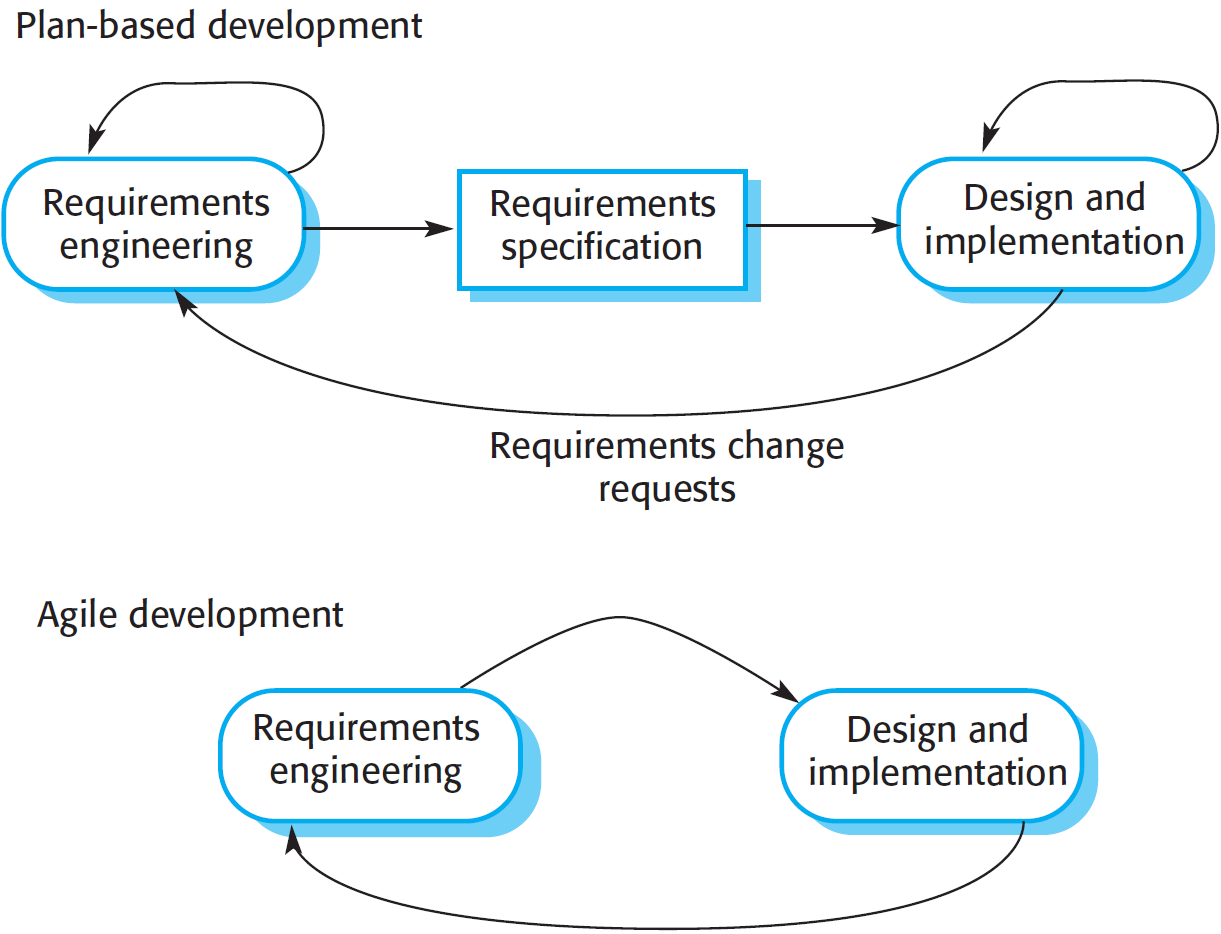
\includegraphics[width=\linewidth]{images/plandriven-and-agil-development.png}
	\caption{Traditionelle und agile Softwareentwicklung \cite{sommerville16}}
	\label{fig:development}
	\Description{}
\end{figure}

\section{Epics und User Stories} \label{def:epics_user_stories}
Wie in dem \emph{Agile Manifesto} \cite{beedle_principles_2001} festgehalten, muss eine agile Softwareentwicklung
auf sich verändernde Anforderungen reagieren können.
Dies führt dazu, dass viele herkömmliche Methoden zur Anforderungsanalyse für diese Art von Softwareentwicklung
nicht mehr geeignet sind.

Um mit diesen Veränderungen im Requirements Engineering umzugehen, sind neue Werkzeuge und Konzepte
für diese Phase der Softwareentwicklung entstanden, welche die Prinzipien der agilen Softwareentwicklung
berücksichtigen und unterstützen.

Das Konzept von \emph{Epics und User Stories} gehört zu diesen neuen Methoden und soll das Entwicklerteam
bei der Anforderungsanalyse unterstützen. Im folgenden Abschnitt werden die zugrundeliegenden Definitionen
dieses Konzeptes vorgestellt, anhand eines Beispiels verdeutlicht und die Vor- und Nachteile beleuchtet.

\subsection{Definition ``User Story''}
\cite[p. 4]{cohn_user_2004} beschreibt ``[e]ine \emph{User Story} [als] eine Funktionalität, welche wertvoll für einen Nutzer [...] eines Systems
oder Software ist''.
Diese Funktionalität wird dabei mit ein bis zwei Sätzen in folgender Struktur formuliert:

\vspace{1em}
\texttt{As a \underline{<type of user>}, I want to \underline{<goal>}\\
	\hspace*{13em} so that \underline{<achieved value>}.}
\begin{flushright}
	\cite[p. 499]{balzert09}
\end{flushright}


\vspace{.5em}

\verb|<Type of user>|, \verb|<goal>| und \verb|<achieved value>| stellen hierbei Platzhalter dar,
welche je nach Anforderung ausgefüllt werden müssen.
\cite{jeffries_essential_2001} unterteilt eine User Story in folgende drei Teile:
\begin{description}
	\item[Card] repräsentiert die Anforderung, strukturiert nach oben genannter Vorlage.
	\item[Conversation] findet als (verbale) Kommunikation der Anforderung zwischen Kunde und Entwickler oder Entwickler und Entwickler statt.
	\item[Confirmation] besteht aus den Akzeptanztests, welche die notwendigen Eigenschaften der Anforderung festlegen.
\end{description}

In vielen Fällen begegnet ein Entwickler der User Story durch die Card.
Diese wird aus Sicht des Kunden formuliert oder sogar von diesem verfasst \cite[p. 497]{balzert09}.

Auf der Card wird in wenigen Sätzen die in der User Story transportierte Anforderung zusammengefasst.
Dabei sei hervorgehoben, dass die Card nicht etwa als vollständige Spezifikation für die geforderte Funktionalität dient,
sondern lediglich als Erinnerung und Grundlage für spätere Diskussion.
Diese wird in der Conversation durchgeführt und gegebenenfalls dokumentiert.
Ziel der Conversation ist es dabei, die Details der Funktionalität zu klären
und durch Akzeptanztests in der Confirmation als Spezifikation für die Implementierung
der Funktionalität festzuhalten \cite[p. 4]{cohn_user_2004}.

% TODO: Wie können Nichtfunktionale Anforderungen in User Stories abgebildet werden?
Aufgrund der Formulierung der Card der User Story, sind Entwicklerteams häufig mit der Herausforderung konfrontiert, wie nichtfunktionale Anforderungen in diesem Konzept abgebildet werden können.
Da nichfunktionale Anforderungen häufig technische Details oder weitreichende Konzepte wie Sicherheit oder Effizienz der Anwendung ansprechen,
besteht die Schwierigkeit darin, die Formulierung so zu wählen, dass der Wert der resultierende User Story für den Kunden immer noch ersichtlich ist.

Eine Lösungsmöglichkeit besteht hier darin das Thema der Story wieder so konkret wie möglich zu wählen und die nichtfunktionale Anforderung in einem
Epic zu verpacken. Zum Beispiel kann ein Epic lauten:

\vspace{1em}
\texttt{Als Professor sollen meine Daten geschützt sein, \\
	\hspace*{5.5em} damit diese nur von mir zugreifbar sind.}
\vspace{1em}

Eine daraus resultierende User Story kann dann konkrete Maßnahmen benennen, die unternommen werden um die Daten von Professoren zu schützen.

Eine andere Möglichkeit um nichtfunktionale Anforderungen in User Stories abzubilden besteht darin, Rollen zu finden, welche ein Interesse daran haben,
dass die nichtfunktionale Anforderung erfüllt wird. Wenn es zum Beispiel um die Effizienz einer Anwendung geht, kann zum Beispiel der Betreiber der
Anwendung als Rolle gewählt werden. Dieser hat ein offensichtliches finanzielles Interesse daran, dass eine Anwendung mit seinen Ressourcen möglichst effizient
umgeht.

Zuletzt können nichtfunktionale Anforderungen auch direkt in den Akzeptanzkritieren, also der Confirmation, mit untergebracht werden.
So kann ein Entwicklerteam zum Beispiel gewisse Standards für den fertigen Quellcode fordern.
Ein anderes weitverbreitetes Beispiel ist die Forderung eines bestimmten Testabdeckunganteils für den neu geschriebenen Code.

\subsection{Definition ``Epic''}
Ein \emph{Epic} stellt eine Vision oder ein übergeordnetes Ziel dar.
Es gleicht in der Formulierung der User Story, umfasst aber einen viel größeren Umfang \cite[pp. 6, 14]{cohn_user_2004}.
Das Epic repräsentiert nämlich nicht nur eine einzelne Anforderung, sondern einen Anforderungsbereich.
Somit bietet es dem Kunden und den Entwicklern eine Orientierungshilfe beim Formulieren der User Stories,
ist aber selber unbrauchbar für die direkte Implementierung von Software-Features.

Um den Zweck einer Vision zu erfüllen, werden Epics dementsprechend grob und allgemein formuliert.
Sie lassen einen weiten Interpretationsspielraum offen, welcher durch weitere Absprachen zwischen
Kunde und Team bzw. innerhalb des Entwicklerteams ausgefüllt werden müssen.

Die Vorlage für die Formulierung von User Stories kann selbstverständlich auch für Epics verwendet werden.
Dies bietet den Vorteil, dass schon die Vision aus der Perspektive des Kunden, bzw. des Stakeholders formuliert
wird. Dies vereinfacht gegebenenfalls das spätere Formulieren von User Stories.

\subsection{Beispiel}
Um das Konzept der \emph{Epics und User Stories} besser zu verdeutlichen, wurden alle Beispiele in diesem
Artikel für ein imaginäres Kursverwaltungssystem erstellt.
Dieses System soll Mitgliedern einer Hochschule die digitale Verwaltung von Kursen und deren zugehörigen Informationen
und Prüfungen ermöglichen.
Außerdem sollen Studierende in der Lage sein, sich zu Kursen, bzw. Prüfungen an- und abzumelden.

Für dieses System wird in diesem Abschnitt am Beispiel eines spezifischen Epics der Umgang mit Epics und User Stories erläutert.

Das Epic ist basierend auf der Vorlage aus dem vorhergehenden Abschnitt formuliert.
Dabei sind die Phrasen, welche für die Platzhalter eingesetzt wurden, unterstrichen.

Das gewählte Epic lautet wie folgt:

\vspace{1em}
\texttt{Als \underline{Professor} möchte ich \underline{meine Kurse digital }\\
	\hspace*{3em}\underline{ verwalten}, damit \underline{die Studierenden }\\
	\hspace*{4em} \underline{ unabhängig mit diesen interagieren können}.}
\vspace{1em}

Wie schon in der Definition des Epics angesprochen handelt es sich bei einem Epic um ein umfangreiches
Arbeitspaket, welches mehr eine Vision oder größeres Ziel ausdrückt, als eine einzelne Anforderung.
Im Beispiel ist dies unschwer durch den Gebrauch von groben Formulierungen zu erkennen. So wird zum
Beispiel lediglich festgelegt, dass ein \underline{\texttt{Professor}} seine \underline{\texttt{Kurse digital verwalten}}
möchte. Diese Formulierung lässt einen großen Spielraum für die spätere Implementierung und erzwingt gleichzeitig
auch die Eingrenzung des Systems durch weitere Anforderungen, damit dieses erfolgreich modelliert und implementiert werden kann.

Einige Fragen, welche das Epic noch offen lässt sind zum Beispiel:

\begin{itemize}[topsep=5pt]
	\item Was bedeutet digital verwalten?
	\item Soll eine Web-, Desktop- oder Mobile-Anwendung entwickelt werden?
	\item Welche Art von Interaktion soll für die Professoren und Studierenden möglich sein?
\end{itemize}

Die Antworten auf diese Fragen stellen weitere Anforderungen an das System dar.
Diese werden wiederum als User Stories formuliert und weiterverarbeitet.
Selbstverständlich können auch hier nocheinmal User Stories entstehen, welche
zu generell sind und deshalb weitere Verfeinerung benötigen.
Tatsächlich handelt es sich dann um ein weiteres Epic, welches wiederum durch den
vorher erläuterten Prozess verfeinert werden muss.
Hierbei ist es allerdings wichtig, dass User Stories nicht bis in das kleinste Detail
aufgeteilt werden dürfen \cite[p. 6]{cohn_user_2004}.
Wie in der Definition erwähnt gehört zu einer User Story neben der \emph{Card}, der Formulierung,
auch die \emph{Conversation}, in welcher die Details der User Story geklärt werden.
Die Absicht User Stories so spezifisch wie möglich zu formulieren würde hier nur zu überflüssiger
Redundanz führen, welche schlussendlich die Effizienz des Entwicklungsteams senkt.

Anhand dieser Überlegungen sind folgende zwei User Stories als Verfeinerung des oben genannten Epics verfasst:

\vspace{1em}
\texttt{Als \underline{Professor} möchte ich \underline{die Kursverwaltung per }\\
	\hspace*{2em} \underline{ Weboberfläche bedienen können}, damit\\
	\hspace*{6em} \underline{ich von unterschiedlichen Geräten }\\
	\hspace*{14em} \underline{ darauf zugreifen kann.}}
\vspace{1em}

Diese User Story geht auf die ersten beiden Fragen ein und stellt eine in diesem Punkt
eine Spezialisierung der Anforderung dar.

Hierbei sei anzumerken, dass es ausgehend von dem Epic keine eindeutig richtige oder
falsche Spezialisierung gibt.
In diesem konkreten Fall wären alle drei Möglichkeiten,
nämlich eine Web-, Desktop- oder Mobile-Anwendung zu entwickeln, korrekt gewesen.
Das Epic lässt die Interpretation von \emph{digital} offen.

Aus diesem Grund wird in vielen Fällen für die Spezialisierung des Epics weitere Kommunikation
mit dem Kunden des Systems von Nöten sein.
Meist kann nur dieser die korrekte Interpretation der Anforderung liefern.

Wie und ob diese Kommunikation stattfindet ist allerdings Sache des (agilen) Vorgehensmodells, welches
das Entwicklerteam anwendet.

\vspace{1em}
\texttt{Als \underline{Professor} möchte ich \underline{die Kursinformationen }\\
	\hspace*{4.5em} \underline{ verändern können}, damit \underline{sie richtig} sind.}
\vspace{1em}

In dieser zweiten User Story findet eine Spezialisierung der dritten Frage statt.
Bei dieser Frage geht es nicht darum, die Mehrdeutigkeit eines verwendeten Begriffs zu klären,
sondern konkrete Beispiele aus einem durch das Epic aufgespannten Anforderungsbereich
zu formulieren.

So könnten in Zukunft noch weitere User Stories hinzukommen, die das Epic in Bezug auf die dritte
Frage spezialisieren.
Zum Beispiel könnte eine weitere User Story eine mögliche Interaktion der Studierenden beschreiben:

\vspace{1em}
\texttt{Als \underline{Studierender} möchte ich \underline{mich für die Teilnahme }\\
	\hspace*{2em}\underline{ an einem Kurs registrieren },\\
	\hspace*{4em}damit \underline{mir diese Teilnahme angerechnet wird}.}
\vspace{1em}

\subsection{Was sind gute User Stories?}
Die Definition von User Stories und Epics beschreibt die Struktur und die Rahmenbedingungen bei der Erstellung einer User Story.
In der Praxis bleibt ausgehend von dieser Definition aber die Frage offen, welche Merkmale eine gute User Story aufweist.

\cite{wake_invest_2003} hat für diesen Zweck sechs Eigenschaften für eine gute User Story unter dem Akronym \textbf{INVEST} zusammengefasst.
\begin{description}[topsep=5pt]
	\item[Independent:] Eine gute User Story ist nicht von anderen User Stories abhängig.
	\item[Negotiable:] Eine gute User Story stellt keine unveränderbare Spezifikation dar, sondern dient als Diskussionsgrundlage.
		Die Implementationsdetails werden nicht vorher festgelegt, sondern über den Lebenszyklus der User Story als Teil der Conversation
		erarbeitet.
	\item[Valuable:] Eine gute User Story stellt einen Mehrwert für den Kunden dar.
	\item[Estimatable:] Der Aufwand einer guten User Story ist schätzbar.
	\item[Small:] Eine gute User Story ist klein und umfasst nur eine einzelne Anforderung, welche in kurzer Zeit implementiert werden kann.
	\item[Testable:] Die Erfüllung einer guten User Story ist prüfbar.
\end{description}


\section{Agile Vorgehensmodelle} \label{sec:agile-vorgehensmodelle}

\emph{RE} und die Verwendung von User Stories und Epics wird in verschiedenen Projektmanagementmethoden unterschiedlich gehandhabt. Im Folgenden werden
diese Aspekte in den agilen Modellen Kanban, Scrum und Feature-driven Development betrachtet und die Vorgehensweisen bewertet. Dabei wird auch auf die Unterschiede eingegangen.
Weiterhin werden für einige Herausforderungen, die bei der Arbeit mit User Stories entstehen, konkrete Lösungsmethoden vorgestellt.

\subsection{Requirement Engineering in Kanban}

Für das \emph{RE} in Kanban wird dem Team viel Spielraum gelassen,
um seine eigenen Methoden und Vorgehensweisen zu entwickeln. Anders als bei Scrum, sind
in Kanban keine spezifischen Rollen für einzelne Teammitglieder vorgesehen. Eine
Spezialisierung einzelner Mitglieder auf bestimmte Bereiche, wie bspw. das \emph{RE}, ist trotzdem
möglich.

In Kanban wird vorgesehen, dass die Requirements und Epics in enger Zusammenarbeit mit
den Stakeholdern erarbeitet werden. Dabei ist für den Austausch mit diesen keine
spezifische Rolle oder Methodik vorgesehen, sodass meist ein oder mehrere Teammitglieder
diese Aufgabe dynamisch übernehmen können. \cite{agileprocesses}

Die zu den Epics gehörenden User Stories werden meist in enger Zusammenarbeit im Team erstellt,
geschätzt, priorisiert und ihre \emph{Akzeptanzkriterien} festgelegt. Dazu steht dem Team eine Vielzahl
von Methoden zur Verfügung. Einige dieser Methoden werden im Verlauf des Kapitels vorgestellt.
Es wird dabei oft versucht die entstehenden User Stories so zu konzipieren, dass sie als vertikale
Scheibe des Gesamtsystems umgesetzt werden können. Das bedeutet, dass ein eigenständiges, vorzeigbares
Produkt entsteht, das sich durch die gesamte Architektur des Systems zieht. Dies ist allerdings
vor allem in komplexen Systemen nicht immer möglich oder einfach zu aufwändig. Die technischen Details für die Implementierung
der User Stories werden in Teams geklärt, damit die relevanten Teammitglieder sich auf eine Vorgehensweise
einigen können. \cite{agileprocesses}

Wie größere User Stories in Kanban heruntergebrochen und welche Methoden dafür genutzt werden, bleibt
dem Team vollständig überlassen. Eine Methode, die man dafür verwenden kann, wird in Kapitel \ref{sec:breakedown} vorgestellt.
Der Zeitaufwand für eine User Story sollte am Ende ein paar Tage betragen, aber nicht mehrere Wochen übersteigen, damit die User Stories besser
geplant und auf einem Kanban-Board verwendet werden können. Gegebenenfalls kann das Team auch entscheiden eine User Story in Tasks, also noch
kleinere Aufgaben, aufzuteilen. Diese können bereits etwas technischer orientiert sein. \cite{agileprocesses}

\begin{figure}[t]
	\centering
	\includegraphics[width=\linewidth]{images/Kanban-Board-mit-userstories-groß.png}
	\caption{Kanban Board mit User Stories}
	\label{fig:kanban-board}
	\Description{}
\end{figure}

In Kanban werden die User Stories auf einem Kanban-Board visualisiert. Auf diesem werden sie je nach Bearbeitungszustand verschiedenen
Listen zugeordnet (siehe Abb. \ref{fig:kanban-board}). Meist werden die User Stories in den einzelnen
Zuständen nach ihrer Priorität geordnet. In Kanban kann der Inhalt des Kanban-Boards zu jeder Zeit verändert werden.
So können User Stories von dem Board entfernt, angepasst, oder bei Bedarf in kleinere User Stories oder Tasks aufgeteilt werden. So kann das Team sehr schnell
auf Änderungen reagieren. \cite{agileprocesses}

In Kanban liegt es im Ermessen des Teams, wann aus den fertig umgesetzten User Stories ein neuer Release
erstellt wird. So kann das Team flexibel entscheiden, wie lang ein Feedbackloop ist. \cite{agileprocesses}

\subsubsection{Vorteile und Nachteile von Requirement Engineering in Kanban}

Die Art und Weise, wie das \emph{RE} in Kanban durchgeführt wird, ermöglicht es dem Team sehr flexibel zu arbeiten.
Das liegt daran, dass die User Stories jederzeit auf dem Kanban-Board angepasst, entfernt,
hinzugefügt oder umgeordnet werden können. Dadurch kann das Team schnell auf Änderungen wie Bugs und Requirementsänderungen
reagieren. Das Kanban-Board ermöglicht es auch dem Team und dem Stakeholder leichter den Überblick über den
Fortschritt des Projekts zu behalten, und hilft dabei, die Entwicklung zu dokumentieren.

Eine Studie in \emph{``Agile Processes in Software Engineering and Extreme Programming''} \cite{agileprocesses} zeigt, dass ein gutes Team mit Kanban konstant und iterativ entwickeln und sich zusätzlich
an dynamisch verändernde Anforderungen anpassen kann. So wird das Team dazu angeregt, Lösungen aus eigener
Initiative zu entwickeln, ohne an eine feste Ablaufstruktur gebunden zu sein. \cite{reqkanban}

Durch das \emph{RE} in Kanban entstehen allerdings auch einige Herausforderungen für das Team. Aufgrund der flexiblen
Struktur braucht das Team eine große Selbstverantwortung und Teamdisziplin. So muss es selbständig \emph{RE} in den
dynamischen Entwicklungsprozess integrieren. Auch die Kommunikation und den Austausch mit den Stakeholdern muss
das Team passend einplanen. Vor allem bei größeren oder unerfahrenen Teams kann dieser zusätzliche Aufwand für
die Planung der Ablaufstruktur ein größeres Problem darstellen. \cite{kanbannod}

\subsection{Requirement Engineering in Scrum}

Anders als bei Kanban, ist in Scrum für das Team eine dedizierte Phase vor einem Sprint für das \emph{RE} bestimmt. In dieser
beschäftigt sich das Team mit den User Stories für den nächsten \emph{Sprint Backlog}. Diese Phase wird als \emph{Sprint Planning} bezeichnet. \cite{reinscrum}

Ein weiterer Unterschied zu Kanban besteht darin, dass beim \emph{RE} bestimmte vordefinierte Rollen im Team eine
große Bedeutung spielen. So ist z.B. der \emph{Scrum Master} dafür verantwortlich sicherzustellen, dass das Team sich mit den
User Stories ordentlich beschäftigen kann. Die wichtigste Rolle für das \emph{RE} in Scrum ist der \emph{Product Owner}. Dieser ist
dafür verantwortlich den \emph{Product Backlog} zu verwalten. Das bedeutet, dass er für das Formulieren und Herunterbrechen der
Epics und User Stories zuständig ist. Es wird allerdings empfohlen, dass er dafür auch Teile des Teams mit einbezieht. So ist er auch für
das Ermitteln der Requirements der Stakeholder zuständig und dient oft auch als direkter Ansprechpartner für diese. \cite{reinscrum}

Weiterhin ist er dafür zuständig, die User Stories im \emph{Product Backlog} nach ihrer Priorität zu ordnen und auf ihre Machbarkeit
zu kontrollieren. Eine Methode, mit der man User Stories nach ihrer Priorität ordnen kann, wird in Kapitel \ref{sec:priorization} erklärt.
Er soll während des \emph{Sprint Plannings} geeignete User Stories an das Team kommunizieren, um sicherzustellen, dass das Verständnis
des Teams mit dem des Stakeholders vereinbar ist. \cite{reinscrum}

Das Team selbst hat hinsichtlich des \emph{RE} die Aufgaben, während des \emph{Sprint Plannings} die einzelnen User Stories für den \emph{Sprint
	Backlog} auszuwählen und deren Aufwand zu schätzen, sie zu priorisieren und ihre \emph{Akzeptanzkriterien} festzulegen. Eine Methode zum Schätzen des Aufwands, wird in Kapitel \ref{sec:effort} vorgestellt.
Weiterhin muss das Team sich im \emph{Sprint Planning} auf die technischen Details der Implementierung der User Stories einigen. [4]

In Scrum sind Epics ein größeres Themengebiet aus zusammengehörenden Requirements. Sie repräsentieren einen Themenkomplex, der
zu groß ist, um ihn in einem Sprint vollständig zu implementieren. \cite{reinscrum}

\begin{figure}[t]
	\centering
	\includegraphics[width=\linewidth]{images/sprint-burndown2-groß.png}
	\caption{Burndown Chart für einen 2 Wochen Sprint}
	\label{fig:burndownchart}
	\Description{}
\end{figure}

User Stories in Scrum definieren die Ziele eines Sprints und bilden den Inhalt des \emph{Sprint Backlogs}. Sie helfen dem Team dabei den Fortschritt
des Sprints in z.B. einem Burndown Chart zu erfassen. Dabei sollten die User Stories einen kleinen und ähnlichen Umfang haben, sodass
sich die Linie für die Abarbeitung der Story Points eines Sprints an eine linear fallende Linie annähert (siehe Abb. \ref{fig:burndownchart}). So kann das
Team leichter erkennen, ob sie den Zeitplan für den aktuellen Sprint einhalten. Sollte erkannt werden, dass der Sprint nicht planmäßig verläuft, können im
\emph{Daily Scrum} Gegenmaßnahmen eingeleitet werden. Sind die User Stories zu groß gewählt, fällt der
Graph auf dem Burndown Chart gegen Ende des Sprints immer stärker ab, was oft dazu führt, dass zu spät erkannt wird, dass der Zeitplan
nicht eingehalten werden kann (siehe Abb. \ref{fig:burndownchart}). \cite{reinscrum}

Ein grober Richtwert, wie klein die User Stories sein sollten, liefert \emph{``The Humanizing Work Guide to Splitting User Stories''} \cite{humanizingwork}. Hier wird empfohlen, dass die Größe einer User Story in
Scrum zwischen \( \frac{1}{6} \) und \( \frac{1}{10} \) der \emph{Velocity} des Teams liegen soll. Bei der \emph{Velocity} handelt
es sich dabei um die Geschwindigkeit der Entwicklung in einem Sprint. Sie wird oft in Form von Story Points ausgedrückt und wird vor
Beginn des Sprints festgelegt. \cite{humanizingwork}

Bei dem Zusammenstellen des \emph{Sprint Backlogs} sollte darauf geachtet werden, dass die verwendeten User Stories zusammen ein auslieferbares
Produkt bilden, das am Sprint-Ende den relevanten Stakeholdern als neues Release vorgestellt werden kann. Dabei kann sich der Stakeholder
am \emph{Sprint Backlog} orientieren, um besser einzuschätzen, ob das Resultat des Sprints seinen Erwartungen entspricht. \cite{reinscrum}

\subsubsection{Vorteile und Nachteile von Requirement Engineering in Scrum}

Das \emph{RE} in Scrum profitiert von dem klar strukturierten Ablaufplan für jede Iteration. Das \emph{Sprint Planning} ermöglicht es dem Team, sich in einem festgelegten Zeitrahmen
ausschließlich darauf zu konzentrieren, welche User Stories im nächsten Sprint bearbeitet werden und wie deren Umsetzung erfolgt. Das erleichtert es vor
allem bei unerfahrenen Teams, alle Mitglieder auf die gleiche Verständnisebene bezüglich der Ziele des Sprints zu halten. Das Team muss sich
also keine Gedanken darüber machen, wie das \emph{RE} dynamisch in die Entwicklung eingebunden werden soll.

Es ist auch vorteilhaft, dass die Stakeholder in regelmäßigen Abständen über den Fortschritt des Projekts anschaulich informiert werden und
dadurch die Kommunikation mit diesen erleichtert und oft klarer wird. Die festen Iterationsintervalle erleichtern es dem Team, die verwendeten Methoden bei
Bedarf anzupassen, um folgende Sprints zu verbessern. So kann z.B. die Schätzungsmethode zwischen Sprints einfach gewechselt
werden, wenn die aktuelle Methode nicht die geforderte Genauigkeit liefert.
Weiterhin wird ein Großteil des \emph{RE} auf den \emph{Product Owner} übertragen, was es dem restlichen Team ermöglicht, sich stärker auf die Implementierung zu fokussieren.

Zwar erleichtert die feste Ablaufstruktur die Planung des \emph{RE} in Scrum, allerdings wird sie dadurch auch unflexibler. So ist es in Scrum nicht
vorgesehen den \emph{Sprint Backlog} während der Sprintphase anzupassen, was es dem Team erschwert, auf kurzfristige Änderungen zu reagieren. Dies
kann vor allem bei Bugs, integriertem Kundensupport und Customizing zu Problemen mit Stakeholdern führen. Das liegt daran, dass in
diesen Kategorien sehr kurzfristig Anforderungen mit hoher Priorität entstehen können.

Weiterhin hängt der Erfolg eines Sprints stark von der Arbeit ab, die während des \emph{Sprint Plannings} geleistet wurde, da die Ergebnisse aus
dieser Phase während eines Sprints nicht mehr angepasst werden sollen. Dies kann dazu führen, dass ein schwerer Fehler im \emph{Sprint Planning} zum
Abbruch des Sprints führen kann. Ähnliches gilt auch für den \emph{Product Owner}. Dieser nimmt zwar dem restlichen Team einen signifikanten Teil
des \emph{RE} ab, hat aber entsprechend viel Verantwortung. Der Erfolg des Projekts hängt davon ab, dass er die Requirements der Stakeholder korrekt
analysiert und verständlich an das Team kommuniziert.

\subsection{Feature Driven Development}
Im Folgenden wird erläutert, wie Epics und User Stories im Feature Driven Development (FDD) in den Arbeitsprozess integriert sind.

\subsubsection{Überblick über FDD}
Das Konzept des Feature Driven Development wurde erstmals in Kapitel 6 von \cite{coad99} beschrieben.
Im Zentrum dieses Ansatzes steht dabei der Begriff des \emph{Feature}, das dort als ``small client-valued functionality'' definiert wird, also eine Funktionalität, die einen konkreten Nutzen für den Kunden oder Anwender hat.

Ein Feature wird in der folgenden Form beschrieben:

\begin{quote}
	\texttt{<Aktion>\hspace{5ex}<Ergebnis>\hspace{5ex}<Objekt>}
\end{quote}

Ein Beispiel für ein solches Feature ist:

\begin{quote}
	\texttt{Verwalte die Informationen des Kurses.}
\end{quote}

Die Entwicklungszeit eines Features ist auf wenige Stunden bis maximal zwei Wochen beschränkt.

FDD eignet sich besonders gut für große Softwareprojekte mit vielen Entwicklern, die in verschiedene Teams aufgeteilt werden.
Zusätzlich zu den Entwicklungsteams wird ein Planungsteam gebildet, welches aus erfahrenen Softwarearchitekten und Domainexperten besteht.

FDD folgt dabei einem klar strukturierten Prozess, der in fünf Phasen gegliedert ist (siehe Abb. \ref{fig:fdd}). Diese Phasen lassen sich in zwei Bereiche einteilen: die Aufgaben des Planungsteams und die der Entwicklungsteams. Das Vorgehen wird in \cite{coad99} folgendermaßen beschrieben:

Zunächst wird ein Objektmodell der Software entwickelt (\emph{Phase 1: Develop an Overall Model}).
Anschließend wird eine Liste von Features erstellt (\emph{Phase 2: Build a Feature List}).
Darauf aufbauend wird für jedes Feature ein Entwicklungsplan erstellt (\emph{Phase 3: Plan by Feature}).
Jedem Entwicklungsteam werden dann ein oder mehrere Features zugeordnet.
Die Teams erarbeitet zunächst ein Design-Paket für die jeweiligen Features (\emph{Phase 4: Design by Feature}),
anschließend erfolgt die Implementierung (\emph{Phase 5: Build by Feature}).

\begin{figure}[t]
	\centering
	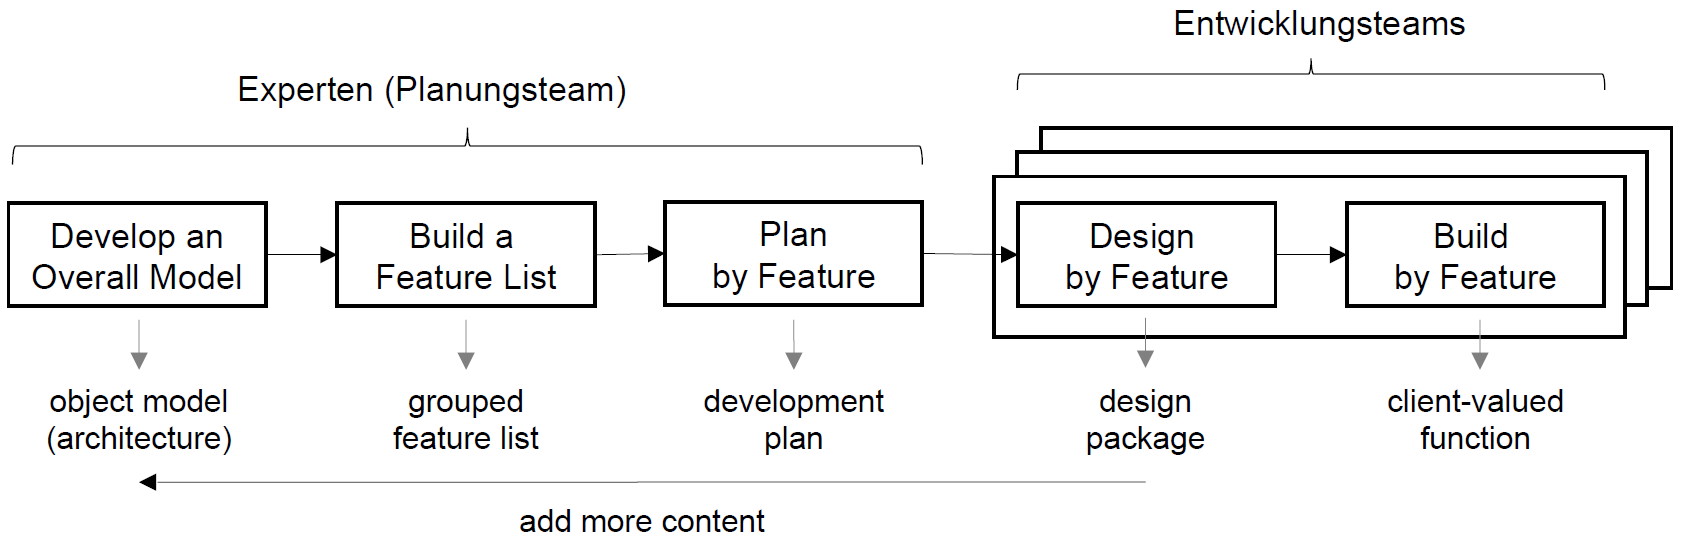
\includegraphics[width=\linewidth]{images/fdd.png}
	\caption{Feature Driven Development}
	\label{fig:fdd}
	\Description{}
\end{figure}

Dieses strukturierte, inkrementelle Vorgehen soll ermöglichen, regelmäßig sichtbaren Fortschritt zu liefern, ohne die Prozesse dabei unnötig zu verkomplizieren \cite{hunt06}.

\subsubsection{Feature vs. User Story}

Sowohl Features als auch User Stories dienen dazu, Anforderungen in überschaubare Teilprobleme zu zerlegen, welche einen konkreten Nutzen für den Anwender haben. Beide sind so formuliert, dass sie für den Kunden und andere Stakeholder verständlich bleiben.

Trotz dieser Gemeinsamkeiten gibt es wesentliche Unterschiede zwischen den beiden Konzepten.
Bereits die unterschiedliche Formulierung zeigt, dass User Stories aus der Sicht des Anwenders formuliert werden, während Features sich primär auf die funktionale Umsetzung konzentrieren.

Ein weiterer Unterschied ist die Vorgabe der Entwicklungszeit.
Bei Features steht die Planbarkeit im Vordergrund \cite{hunt06}, welche durch die Vorgabe von wenigen Stunden bis max. 2 Wochen Entwicklungszeit sichergestellt wird.
In \cite{palmer02} wird zudem betont, dass ein Feature nicht nur eine triviale Methode ist, die lediglich einen Attributwert zurückgibt.
Bei User Stories ist es hingegen durchaus zulässig, auch kleinere Einheiten zu definieren, wie bereits in einigen Beispielen gezeigt wurde.

Weiterhin unterscheidet sich auch die Einbindung in den Entwicklungsprozess.
Während User Stories unter anderem dazu dienen, Objekte und Klassen zu identifizieren, werden Features im Kontext von FDD typischerweise aus der bereits bestehenden Softwarearchitektur bzw. dem Ablaufmodell abgeleitet \cite{palmer02}.

Features und User Stories lassen sich also nicht miteinander vergleichen. Eine User Story kann ein oder mehrere Features enthalten, ein einzelnes Feature kann aber auch in mehreren User Stories vorkommen \cite{hunt06}. Zur Demonstration soll das folgende Beispiel genügen:\smallskip

\begin{tikzpicture}[
		every node/.style={draw, rectangle, font=\footnotesize}]
	\node (us1) [text width=13.2em] {
		\texttt{Als \underline{Studierender} möchte ich \underline{mich}\\
			\underline{für einen Kurs registrieren}, damit\\
			\underline{mir die Teilnahme angerechnet wird}.}
	};
	\node (f1) [right=4em of us1, text width=6.5em] {
		\texttt{Validiere\\
			die Anmeldungen\\
			für einen Kurs.}
	};
	\node (us2) [below=1em of us1, text width=13.2em] {
		\texttt{Als \underline{Professor} möchte ich \underline{die}\\
			\underline{Kursinformationen verändern können},\\
			damit \underline{sie richtig sind}.}
	};
	\node (f2) [right=4em of us2, text width=6.5em] {
		\texttt{Aktualisiere\\
			die Informationen\\
			eines Kurses}.
	};
	\draw [-] (us1.east) -- (f1.west);
	\draw [-] (us1.east) -- (f2.west);
	\draw [-] (us2.east) -- (f2.west);
\end{tikzpicture}

\subsubsection{Rolle von User Stories und Epics in FDD}

Im Gegensatz zu Kanban und Scrum basiert das Konzept des Feature Driven Developments nicht grundlegend auf Epics und User Stories.
Dennoch können sie in Phase 1 bei der Modellierung des Gesamtmodells hilfreich sein.
In den späteren Phasen können sie zudem das Identifizieren von Features unterstützen \cite{hunt06}.
Obwohl die Kommunikation in FDD überwiegend auf Features ausgerichtet ist, bieten User Stories eine nützliche Ergänzung bei der Kommunikation zwischen dem Planungsteam und den Entwicklungsteams sowie zwischen dem Planungsteam und dem Kunden.
Besonders in der Zusammenarbeit mit Stakeholdern sind User Stories hilfreich, da sie die Perspektive des Anwenders stärker in den Vordergrund rücken.
Zudem können sie bspw. in der Dokumentation eines Domain-Walkthroughs eingesetzt werden \cite{palmer02}.

Epics und User Stories übernehmen in FDD üblicherweise nicht die Rolle der Priorisierung und Planung - diese wird durch Features abgedeckt. Stattdessen dienen sie als zusätzliches Hilfsmittel für die Modellierung, Dokumentation und Kommunikation. Diese Rolle sollte allerdings nicht unterschätzt werden, da eine klare und effiziente Kommunikation zwischen dem Planungsteam und den Entwicklungsteams in FDD von entscheidender Bedeutung ist.

Zusammenfassend lässt sich festhalten, dass User Stories und Epics zwar keine zentrale Rolle in FDD einnehmen, aber eine wertvolle Ergänzung darstellen können.

\section{Konkrete Anwendungsmethoden für die Kontrolle von User Stories} \label{sec:konkrete-anwendungsmethoden}

Bei der Betrachtung der agilen Methoden wurde in dieser Arbeit oft darauf hingewiesen, dass die verwendeten User Stories gewisse Kriterien
erfüllen sollten. Zu diesen Kriterien gehört unter anderem, dass die User Story weit genug heruntergebrochen, ihr Aufwand geschätzt und sie priorisiert
wurde. Im Folgenden wird zu diesen Kriterien jeweils eine konkrete Methodik vorgestellt. Weiterhin wird auch noch erläutert, was eine \emph{Definition of
	Ready} (\emph{DoR}) und eine \emph{Definition of Done} (\emph{DoD}) im Zusammenhang mit User Stories ist und wofür sie genutzt werden.

\subsection{Herunterbrechen von User Stories} \label{sec:breakedown}

Eine Methode, um eine zu große User Story richtig herunterzubrechen, wurde von \emph{humanizing Work} veröffentlicht. Dabei handelt es sich um ein Story
Splitting Flowchart, das von Richard Lawrence entwickelt wurde. Diese Methode wurde hauptsächlich für Scrum entwickelt, kann aber auch
in anderen agilen Methoden verwendet werden. \cite{humanizingwork}

Bei dieser Methode wird zunächst geprüft, ob die User Story das \emph{INVEST}-Modell erfüllt. Sollte dies nicht der Fall sein, muss die User Story nochmal
überarbeitet werden. Wenn der geschätzte Aufwand der User Story über dem vordefinierten Bereich liegt (hier zw. \( \frac{1}{6} \) und \( \frac{1}{10} \) der \emph{Velocity}), kann mit dem Herunterbrechen
fortgefahren werden. \cite{humanizingwork}

In dem Flowchart werden dafür verschiedene Kategorien erläutert, nach denen man die User Story weiter herunterbrechen kann. Zu diesen Kategorien
gehören die verschiedenen Arbeitsschritte, genutzte Operationen, Businessregeln, verwendete Datentypen und Schnittstellen. Weiterhin kann man sie auch nach dem größten
Aufwand und der Komplexität unterteilen. Es ist auch möglich, die User Story in Teile aufzuteilen, die bestimmte nichtfunktionale Anforderungen erfüllen müssen,
und solche, die ohne diese Anforderungen auskommen. \cite{humanizingwork}

Nach dem Herunterbrechen nach einer der Kriterien, werden die entstandenen User Stories noch evaluiert. Dabei wird geprüft, ob sie unter anderem das \emph{INVEST}-Modell erfüllen, einen
ähnlichen Aufwand aufweisen, dieser innerhalb des vorgegebenen Bereichs liegt und keine der User Stories redundant ist. Wenn alle Schritte in dem Flowchart richtig umgesetzt wurden,
dann erhält man am Ende gute User Stories mit der gewünschten Größe. \cite{humanizingwork}

\subsection{Aufwandschätzung von User Stories über Planning Poker mit Fibonacci-Zahlen} \label{sec:effort}

Von allen User Stories muss der Aufwand geschätzt werden, um zu bestimmen, ob ihr Umfang sich für das verwendete Projektmodell eignet.
Eine Methode, die man dazu anwenden kann, ist das Planning Poker mit Fibonacci-Zahlen. Dabei wird die Zahlenfolge als der Schätzwert verwendet. \cite{planingpoker}

Sie ist besser für das Schätzen geeignet als eine lineare Zahlenfolge, da die Sprünge zwischen den einzelnen Zahlen nach oben immer größer werden. So kann man
verhindern, dass versucht wird große User Stories unrealistisch genau zu schätzen. Das ist vorteilhaft, weil aus Beobachtungen hervorgegangen ist, dass
die Aufwandschätzung mit zunehmendem Umfang der User Story immer ungenauer wird. \cite{planingpoker}

Das Planning Poker folgt einem festen Ablaufplan. Im ersten Schritt wird die User Story zunächst dem Team präsentiert. Daraufhin wird sie im Team diskutiert,
damit ein einheitliches Verständnis entsteht. Im dritten Schritt schätzt dann jedes Mitglied den Aufwand mithilfe der Fibonacci-Zahlen. Welcher Aufwand genau
geschätzt wird, ist dem Team überlassen. Es können beispielsweise die Story Points oder die Komplexität der User Story geschätzt werden. \cite{planingpoker}

Anschließend werden die Ergebnisse der Schätzungen präsentiert und die Teammitglieder mit der größten Differenz stellen die Gründe für ihre Schätzung vor.
Die Abweichungen werden dann im Team diskutiert. Dabei wird versucht einen gemeinsamen Kompromiss zu finden. Wenn sich das Team in der Diskussion einigen kann, dann wird die Schätzung finalisiert.
Dafür kann man z.B. den Median oder Mittelwert aller Schätzungen bilden. Die verwendete Methode bleibt dabei dem Team überlassen. Sollte sich das Team nicht einigen können, muss der Prozess wiederholt werden. \cite{planingpoker}

\subsection{Priorisieren von User Stories mit MoSCoW-Methode} \label{sec:priorization}

User Stories müssen priorisiert werden, damit sie richtig zugewiesen und eingeplant werden können. Dabei müssen die Abhängigkeiten von User Stories untereinander
beachtet werden, wenn diese vorhanden sind. Für die Priorisierung kann man z.B. die \emph{MoSCoW}-Methode verwenden. Dabei werden die User Stories in vier Kategorien eingeteilt. \cite{moscow}

Dazu gehören als erstes die \emph{Muss}-Kategorie (\emph{Must}). In diese werden User Stories eingeordnet, die absolut essentiell für die Grundfunktionalität sind und ohne die das
Projekt nicht auskommt. In die \emph{Soll}-Kategorie (\emph{Should}) kommen User Stories, die noch durchaus viel Wert für die Stakeholder aufweisen, aber nicht unmittelbar zur Grundfunktionalität
des Produkts gehören und somit nicht unbedingt direkt in der ersten Version umgesetzt werden müssen. Als drittes gibt es die \emph{Kann}-Kategorie (\emph{Could}). Die User Stories in dieser Kategorie sind oft
nützlich, haben aber für den Stakeholder einen eher geringeren Wert. Sie werden oft auch als \emph{``Nice to have''} bezeichnet. Die letzte Kategorie ist die \emph{Nicht}-Kategorie
(\emph{Will not}). In diese fallen die User Stories, die außerhalb des Scopes liegen und höchstens in zukünftigen Versionen von Bedeutung sein könnten. \cite{moscow}

Die erfolgreiche Kategorisierung der User Stories ist bei dieser Methode stark von einer präzisen Aufwandschätzung abhängig. \cite{moscow}

\subsection{Definition of Ready und Definition of Done}

Damit das Team erkennt, wann eine User Story bereit für die Bearbeitung, oder fertig implementiert ist, definieren die meisten Unternehmen eine \emph{DoR} und eine \emph{DoD}.
Bei einer \emph{DoR} handelt es sich dabei um eine Liste von Kategorien, die alle User Stories erfüllen müssen, bevor sie für die Umsetzung freigegeben wird. Der genaue Inhalt
ist bei der \emph{DoR} und der \emph{DoD} dem Unternehmen überlassen. In dem \emph{DoR} könnten durchaus folgende Kriterien enthalten sein:
\begin{itemize}
	\item das INVEST-Modell ist erfüllt
	\item der Aufwand wurde geschätzt und ist innerhalb des vordefinierten Bereichs
	\item die Priorisierung wurde durchgeführt
	\item die \emph{Akzeptanzkriterien} sind festgelegt
	\item die technischen Details sind geklärt
\end{itemize}

Die \emph{Akzeptanzkriterien} (auch \emph{Confirmation} genannt) sind zwischen den verschiedenen User Stories durchaus unterschiedlich.
Sie werden oft von Stakeholdern vorgegeben, können aber auch nichtfunktionale Anforderungen enthalten, oder von dem erfolgreichen
Abschluss vordefinierter Tests (z.B. Unit-Tests) abhängen.

In der \emph{DoD} werden die Kriterien aufgelistet, die alle User Stories erfüllen müssen, damit sie als vollständig umgesetzt gelten. Zu diesen Kategorien können unter anderem
folgende gehören:
\begin{itemize}
	\item das Erfüllen der \emph{Akzeptanzkriterien}
	\item das Dokumentieren der Änderungen
	\item der erfolgreiche Abschluss aller Tests
	\item die Abnahme durch den \emph{Product Owner} oder Projektleiter
\end{itemize}

\subsection{Automatische Verarbeitung von User Stories am Beispiel von Cucumber}
Epics und User Stories werden, ausgehend von der Definition in \ref{def:epics_user_stories}, immer in einer bestimmten Struktur formuliert.
Diese Struktur unterstützt nicht nur menschliche Leser, sondern ermöglicht auch die computergestützte Weiterverarbeitung der User Story.
Ein Beispiel, wo dies zum Einsatz kommt, ist die Software \emph{Cucumber}.

``Cucumber ist ein Tool um Akzeptanztests, welche in verständlicher Sprache verfasst sind, automatisiert auszuführen'' \cite{the_cucumber_open_source_project_cucumber_2025}.
Mit Hilfe von Cucumber ist es möglich sogenannte \emph{Features} in einer von aktuell 80 gesprochenen Sprachen zu verfassen.
Dabei muss lediglich die simple Gherkin-Grammatik eingehalten werden.

Basierend auf diesen Features kann Cucumber dann automatische Akzeptanztests für das jeweilige Feature durchführen.
Insbesondere können durch diese automatisierte Testerzeugung auch neu erstellte User Stories direkt mit dem bestehenden System
überprüft werden. Dadurch kann direkt erkannt werden, an welchen Teilen einer User Story noch Implementationsbedarf besteht und welche
Teile möglicherweise schon durch bestehenden Quellcode abgedeckt sind.

\subsubsection{Workflow an einem Beispiel}
In diesem Abschnitt wird für eine im vorhergehenden Kapitel formulierte User Story beispielhaft eine Umsetzung
mit der Gherkin-Syntax und Cucumber durchgeführt.
Die gewählte User Story lautet:

\texttt{Als Professor möchte ich die Kursinformation \\verändern können, damit sie richtig sind.}

Um diese User Story in der Gherkin-Grammatik auszudrücken, muss lediglich folgendes Schema befolgt werden.

\vspace*{-1em}
\begin{listing}[!h]
	\begin{tcolorbox}[colframe=black, colback=white, opacityback=1.0, sharp corners, boxrule=.4pt, width=\linewidth]
		\vspace*{-.6em}
		\begin{minted}[autogobble, xleftmargin=-12pt, xrightmargin=-18pt]{cucumber}
    Feature: <Titel der User Story>

    Scenario: <Card der User Story>
        Given <Vorbedingung für den Test>
        When  <Veränderung, die getestet werden soll>
        Then  <Akzeptanzbedingung des Tests>
    \end{minted}
		\vspace*{-.6em}
	\end{tcolorbox}
	\vspace*{-1em}
\end{listing}

\vspace*{-1em}
Wie dieses Schema für die oben genannte User Story umgesetzt werden kann, ist in Listing \ref{listing:1} zu sehen.

\begin{listing}[!h]
	\begin{tcolorbox}[colframe=black, colback=white, opacityback=1.0, sharp corners, boxrule=.4pt, width=\linewidth]
		\vspace*{-.6em}
		\inputminted[xleftmargin=-12pt, xrightmargin=-18pt]{cucumber}{cucumber/course_modification.feature}
		\vspace*{-1em}
	\end{tcolorbox}
	\vspace*{-1em}
	\caption{\texttt{course\_modification.feature}}
	\label{listing:1}
\end{listing}


\begin{listing}[!h]
	\begin{tcolorbox}[colframe=black, colback=white, opacityback=1.0, sharp corners, boxrule=.4pt, width=\linewidth-.8pt]
		\vspace{-.6em}
		\inputminted[linenos, firstline=9, breakafter=_, xleftmargin=2pt, numbersep=6pt, frame=none]{java}{cucumber/StepDefinitions.java}
		\vspace{-1em}
	\end{tcolorbox}
	\vspace{-1em}
	\caption{\texttt{StepDefinitions.java}}
	\label{listing:2}
\end{listing}

Um basierend auf solch einer Feature-Datei nun automatisierte Tests durchzuführen, müssen für die einzelnen Testabschnitte
\texttt{Given}, \texttt{When}, \texttt{Then} nun noch Template-Testfunktionen implementiert werden, welche bei der Testdurchführung
die in der Feature-Datei spezifizierten Parameter, in diesem Fall die Strings \texttt{"Software Enginearing"} und
\texttt{"Software Engineering"}, übergeben bekommen.
Der für diesen Zweck im Beispiel verwendete Quellcode ist in Listing \ref{listing:2} zu finden.

Das hier vorgestellte Beispiel und der zugehörige Quellcode sind online auf GitHub in folgenden Repository verfügbar:
\url{https://github.com/Beleg-01-Requirements-Engineering/cucumber-example}.
Dort ist ebenfalls eine Anleitung zum Ausführen der Tests zu finden.


\section{Diskussion} \label{sec:diskussion}
% In diesem Kapitel werden nun nocheinmal die wichtigsten Erkenntnisse dieser Arbeit zusammengetragen.
% Dabei sei zu beachten, dass insbesondere die Auswahl und Bewertung der Erkenntnisse zunächst als Meinung
% der Autoren betrachtet werden sollte. Diese findet zwar ihren Ursprung selbstverständlich in den Ergebnissen der Recherche,
% allerdings ist die Einordnung und Bewertung von Ergebnissen, insbesondere im Bereich des Software Engineering, oft subjektiv behaftet.
% Dies ist auf die Komplexität der Durchführung von eindeutigen Experimenten zurückzuführen.

% Im Rahmen dieser Arbeit wurden die Methode von Epics und User Stories vorgestellt.
% Dabei wurde auf Vorteile und aber auch auf Herausforderungen, welche beim Einsatz dieser Methode für das Requirements Engineering auftreten, eingegangen.
% Dies wurde beispielhaft anhand der drei agilen Vorgehensmodelle Kanban, Scrum und Feature Driven Development erörtert.

Epics und User Stories sind eine Methode, welche für Requirements Engineering im Sinn des Agilen Manifests \cite{agile_manifesto_2001} geeignet sind.
Dies kann durch folgende drei Grundsätze des Agilen Manifests verdeutlicht werden.

\subsection{Individuals and interactions over processes and tools}
Epics und User Stories tragen zu einer klaren Kommunikation sowohl im Team (intern) als auch zwischen Kunde und Entwicklerteam (extern) bei.
Dies zeigt sich auch häufig darin, dass durch den Einsatz von User Stories die Perspektive des Kunden besser verstanden werden kann,
da dieser tief in den Prozess der Anforderungsanalyse involviert ist.

\subsection{Customer collaboration over contract negotiation}
Wie schon im vorhergehenden Punkt angesprochen ist der Kunde beim Erstellen und Bearbeiten von User Stories fest mit eingebunden.
In traditionellen Methoden der Anforderungsanalyse werden häufig Anforderungen einmalig erstellt und dann vertraglich festgesetzt.
Im Gegenteil dazu werden bei User Stories Anforderungen auch nach ihrer Erstellung noch bearbeitet.
Ganz nach dem Qualitätsmerkmal ``Negotiable'' der INVEST-Kriterien, werden mit User Stories
immer wieder durch Kommunikation mit dem Kunden Details erarbeitet oder Teile der User Story angepasst, da sich die zugrundeliegenden
Anforderungen von Seiten des Kunden verändert haben.

\subsection{Responding to change over following a plan}
Zuletzt befähigen Epics und User Stories auch agile Entwicklungsteams auf sich verändernde Anforderungen zu reagieren.
Im letzten Abschnitt wurde schon die Kommunikation zum Kunden als wichtiges Mittel zur Reaktion auf Veränderungen erwähnt.
Darüber hinaus bieten User Stories aber auch durch ihre Größe eine geeignete Struktur für ein Entwicklungsteam, um einerseits
Anforderungen für die Implementation auszuwählen, aber auch in regelmäßigen Zeitabständen den Kunden über den
Stand des Projektes zu informieren und auf dessen Rückmeldung zu reagieren.

Trotz der wesentlichen Vorteile von Epics und User Stories sollen hier auch nocheinmal einige Herausforderungen aufgeführt
werden, auf welche Entwicklungsteams bei ihrem Einsatz stoßen werden.

Wie schon bei der Einführung von Epics und User Stories erwähnt, ist das Formulieren von nichtfunktionalen Anforderungen als User Stories
schwierig. Es gibt Techniken, die dieses Problem lösen, doch erfordert deren Einsatz ein Bewusstsein für diese Herausforderung und ein Verständnis dieser Techniken.

Außerdem besteht die Gefahr der Überspezialisierung auf einen bestimmten Kunden.
Wenn im Rahmen der Anforderungsanalyse ein Großteil der User Stories nur von einem einzelnen Kunden formuliert wird,
können dadurch Anforderungen, welche nur dieser eine Kunde hat, überbewertet und Anforderungen von anderen Kunden unterbewertet werden.
Auch die Anforderungen, welche möglicherweise durch andere Stakeholder der Software (Maintenance, Deployment etc.) an die Software gestellt werden
können in diesem Prozess untergehen.

Der effiziente Einsatz von Epics und User Stories erfordert an vielen Stellen Erfahrung.
Dies kann insbesondere beim Schätzen und Herunterbrechen von User Stories zu Effizienzeinbußen
in unerfahrenen Teams führen. Ein einfaches Mittel, dem entgegenzuwirken, ist Teammitglieder mit unterschiedlichen
Erfahrungsstufen zusammenzustellen und einen aktiven Wissenstransfer anzuregen.

\section{Zusammenfassung} \label{sec:zusammenfassung}
Im Rahmen dieser Arbeit wurden Epics und User Stories als Methode des agilen Requirements Engineering vorgestellt.

Der korrekte Umgang mit User Stories wurde theoretisch anhand des INVEST-Modells erörtert und exemplarisch
an den drei verschiedenen agilen Vorgehensmodellen Kanban, Scrum und Feature Driven Development dargestellt.
Dabei wurden auch mit dem Einsatz von Epics und User Stories verbundene Herausforderungen angesprochen und mögliche
Lösungsmethoden vorgeschlagen.

Zuletzt wurden die Erkenntnisse dieser Arbeit ausgewertet und die Bedeutung von Epics und User Stories für die agile Softwareentwicklung
diskutiert.
Basierend auf dieser Diskussion kommen wir zu dem Schluss, dass Epics und User Stories ein geeignetes Mittel für das
Requirements Engineering in agilen Softwareprojekten sind und wesentlich zu deren Erfolg beitragen.



\bibliographystyle{ACM-Reference-Format}
\bibliography{01-Requirements-Engineering}

\appendix

\section{Anhang 1}

\subsection{Übungsaufgaben}
\subsubsection{Epics und User Stories}\label{aufg:epics-und-user-stories}
Ein Lebensmittelverwaltungssystem soll Privatpersonen helfen ihre gelagerten Lebensmittel abzurufen,
den Lebensmittelverbrauch zu überwachen und bei der Essensplanung unterstützen.

Finden Sie eine geeignete Anforderung für dieses System, welche einem Epic entspricht und formulieren Sie drei zugehörige
User Stories mit Hilfe der Gherkin-Grammatik!

\subsubsection{FDD und nichtfunktionale Anforderungen}
Formulieren Sie für jede Ihrer User Stories aus Aufgabe \ref{aufg:epics-und-user-stories} ein oder mehrere Features in der für FDD typischen Form, die für deren Umsetzung erforderlich sind. Die Wiederverwendung von Features ist erlaubt und sogar erwünscht. Falls sich für eine User Story kein passendes Feature formulieren lässt, begründen Sie dies.

Überlegen Sie außerdem, welche nichtfunktionalen Anforderungen bei der Implementierung der Features berücksichtigt werden sollten.

\subsubsection{User Story herunterbrechen}
Die folgende User Story wurde für die Entwicklung eines typischen Online-Shops erstellt. Nutzen Sie die in Kapitel \ref{sec:breakedown} definierte Methode,
um diese User Story in kleinere herunterzubrechen. Verwenden Sie dazu eine passende Kategorie aus dem Flowchart aus ``\emph{The Humanizing Work Guide to Splitting User Stories}'' (\url{https://www.humanizingwork.com/the-humanizing-work-guide-to-splitting-user-stories/}) \cite{humanizingwork}.
Achten Sie darauf, dass die entstehenden User Stories einen relativ ähnlichen Umfang haben sollen.

User Story:
``Als Benutzer muss ich in der Lage sein, Produkte zu suchen, auszuwählen, in den Warenkorb zu legen und den Kauf abzuschließen, damit ich sie online einkaufen kann.''

\end{document}
\endinput
